There are two main types of lung cancer:
\begin{itemize}
    \item \textcolor{red}{Small Cell Lung Cancer} (SCLC)
    \item \textcolor{red}{Non Small Cell Lung Cancer} (NSCLC)    
\end{itemize}
\section {Small Cell Lung Cancer (SCLC)}

SCLC is a fast-growing cancer that spreads much more quickly than other types of lung cancer. In most people with SCLC, the cancer has already spread beyond the lungs at the time it is diagnosed. Unfortunately, for most people the cancer will return at some point. SCLC are also classed as \textcolor{red}{neuroendocrine tumours} (NETs). Neuroendocrine tumours are rare tumours that develop in cells of the \textcolor{red}{neuroendocrine system}. In small cell lung cancer, the tumour starts in the \textcolor{red}{neuroendocrine cells} of the lung.

\colorbox{green}{Almost all cases of small cell lung cancer are due to cigarette smoking}. Around \textcolor{red}{15 to 20} out of every 100 lung cancers diagnosed are this type. There are two different types of small cell lung cancer:

\begin{itemize}
    \item \textcolor{red}{small cell carcinoma} (also called \textcolor{red}{oat cell carcinoma})
    \item \textcolor{red}{combined small cell carcinoma}.
\end{itemize}

The types of small cell lung cancer are named for the kinds of cells found in the cancer and how the cells look when viewed under a microscope. 

\section{Non Small Cell Lung Cancer (NSCLC)} 
This type of cancer usually grows and spreads to other parts of the body more slowly than small cell lung cancer does. Around \textcolor{red}{80 to 85} out of 100 lung cancers are non small cell lung cancer (NSCLC). There are three different types of NSCLC:-
\begin{itemize}
    \item \textcolor{red}{Adenocarcinoma}
    \item \textcolor{red}{Squamous cell carcinoma}
    \item \textcolor{red}{Large cell carcinoma}
\end{itemize}

\begin{enumerate}
    \item \textbf{Adenocarcinoma} A form of NSCLC often found in an outer area of the lung. It develops in the cells of epithelial tissues, which line the cavities and surfaces of the body and form glands.

    \item \textbf{Large cell carcinoma} A form of NSCLC usually found in the center of the lung next to an air tube (bronchus).

    \item \textbf{Squamous cell carcinoma} A form of NSCLC that can occur in any part of the lung and tends to grow and spread faster than adenocarcinoma or squamous cell carcinoma.
\end{enumerate}



\begin{figure}[ht!]
    \centering
    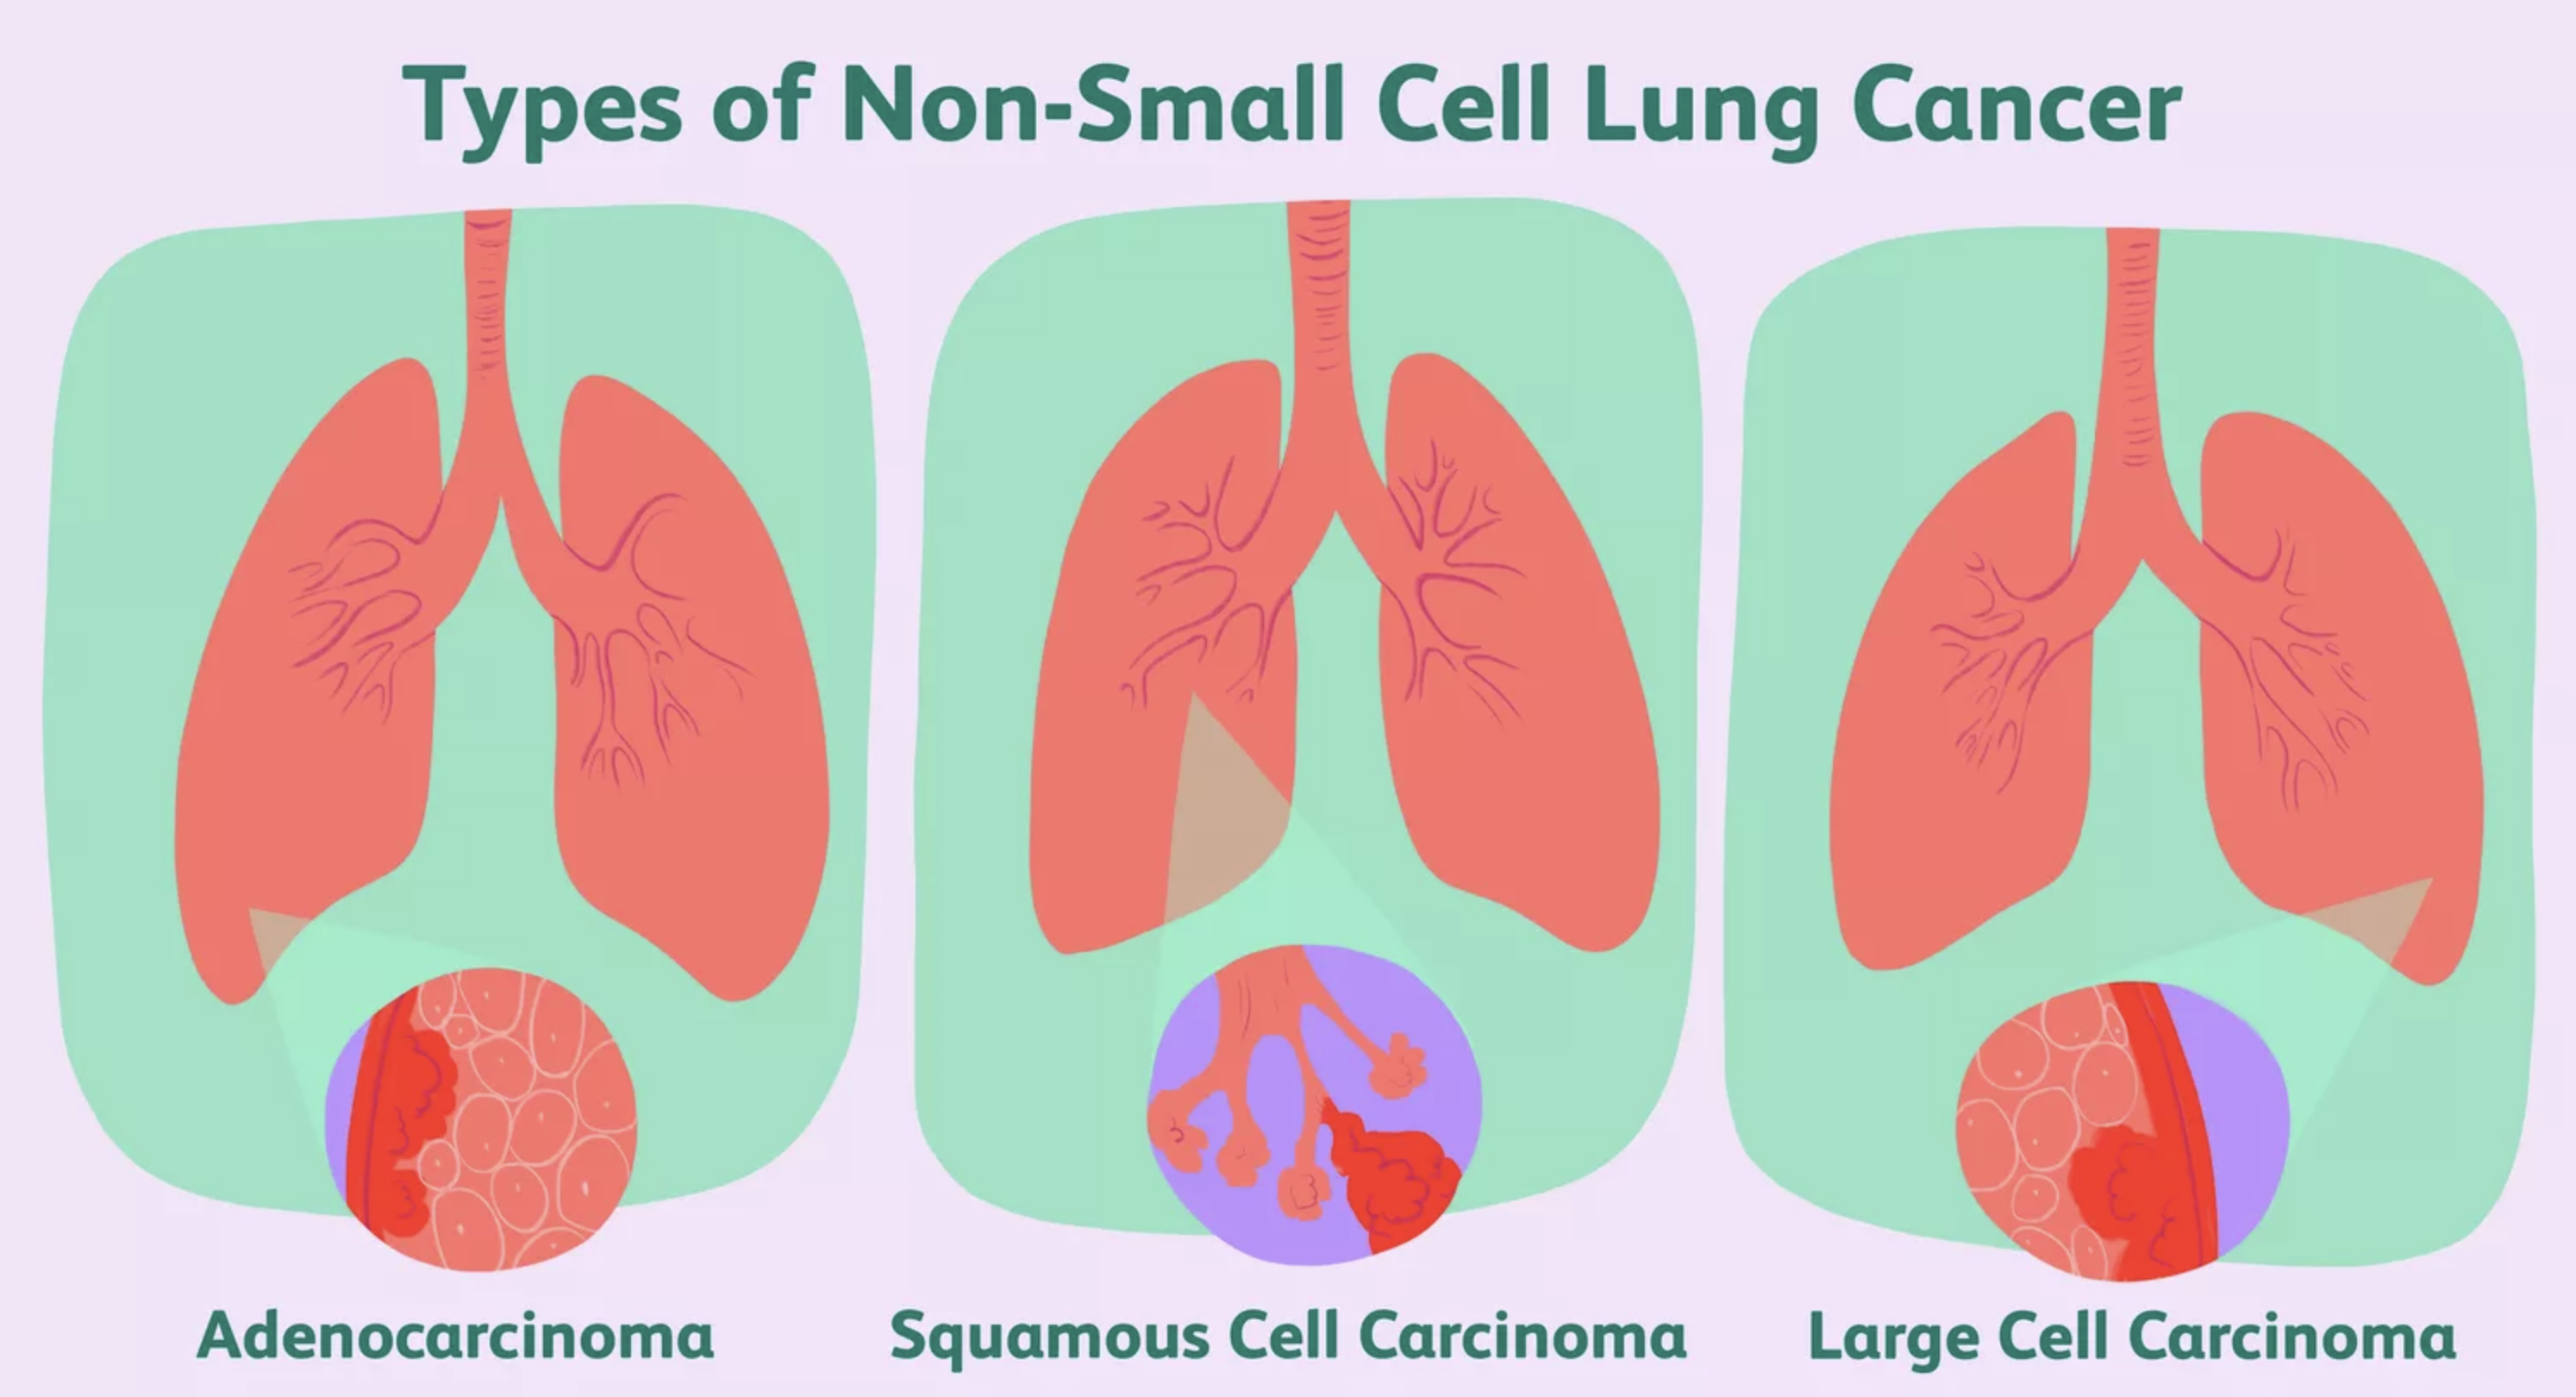
\includegraphics[width=\linewidth]{images/Non_small_cell_lung_cancer.png}
    \caption{Types of Non-Small cell Lung Cancer}
\end{figure}

\section{Other cancers affecting the lungs} 
There are other types of tumors found in the lung. They are rare. Examples are:- \textcolor{red}{\textbf{Salivary gland type tumors, Lung sarcoma, Lung lymphoma }}.
  
\vspace{3.22 mm}
Now lets have a look in the given diagram about percentage of different types of lung cancer:-

\begin{figure}[h!]
    \centering
    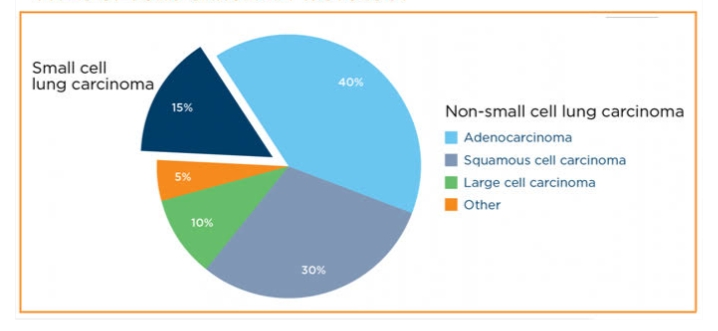
\includegraphics[width= 0.675\linewidth]{images/percentage_of_lc.jpeg}
    \caption{Percentage of different types of lung cancer}
    \label{fig:types-label}
\end{figure}
